% Title: gl2ps_renderer figure
% Creator: GL2PS 1.4.0, (C) 1999-2017 C. Geuzaine
% For: Octave
% CreationDate: Tue Oct 26 17:59:29 2021
\setlength{\unitlength}{1pt}
\begin{picture}(0,0)
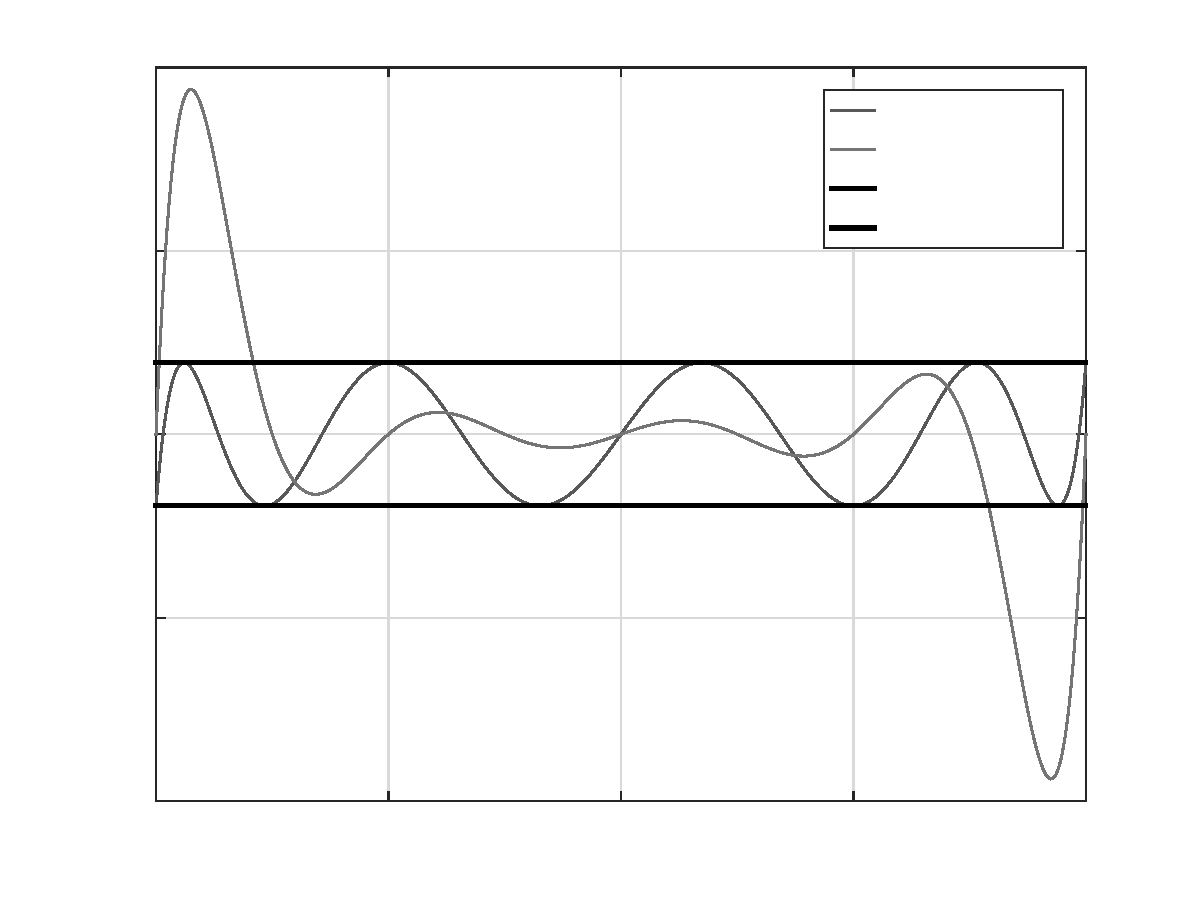
\includegraphics{figures/chap10/OUT/OmegaPlotGray-inc}
\end{picture}%
\begin{picture}(576,432)(0,0)
\fontsize{10}{0}
\selectfont\put(74.88,40.0183){\makebox(0,0)[t]{\textcolor[rgb]{0.15,0.15,0.15}{{-1}}}}
\fontsize{10}{0}
\selectfont\put(186.48,40.0183){\makebox(0,0)[t]{\textcolor[rgb]{0.15,0.15,0.15}{{-0.5}}}}
\fontsize{10}{0}
\selectfont\put(298.08,40.0183){\makebox(0,0)[t]{\textcolor[rgb]{0.15,0.15,0.15}{{0}}}}
\fontsize{10}{0}
\selectfont\put(409.68,40.0183){\makebox(0,0)[t]{\textcolor[rgb]{0.15,0.15,0.15}{{0.5}}}}
\fontsize{10}{0}
\selectfont\put(521.28,40.0183){\makebox(0,0)[t]{\textcolor[rgb]{0.15,0.15,0.15}{{1}}}}
\fontsize{10}{0}
\selectfont\put(69.8755,47.52){\makebox(0,0)[r]{\textcolor[rgb]{0.15,0.15,0.15}{{-0.02}}}}
\fontsize{10}{0}
\selectfont\put(69.8755,135.54){\makebox(0,0)[r]{\textcolor[rgb]{0.15,0.15,0.15}{{-0.01}}}}
\fontsize{10}{0}
\selectfont\put(69.8755,223.56){\makebox(0,0)[r]{\textcolor[rgb]{0.15,0.15,0.15}{{0}}}}
\fontsize{10}{0}
\selectfont\put(69.8755,311.58){\makebox(0,0)[r]{\textcolor[rgb]{0.15,0.15,0.15}{{0.01}}}}
\fontsize{10}{0}
\selectfont\put(69.8755,399.6){\makebox(0,0)[r]{\textcolor[rgb]{0.15,0.15,0.15}{{0.02}}}}
\fontsize{9}{0}
\selectfont\put(422.747,379.182){\makebox(0,0)[l]{\textcolor[rgb]{0,0,0}{{$\omega_9(x)$ (Chebyshev)}}}}
\fontsize{9}{0}
\selectfont\put(422.747,360.318){\makebox(0,0)[l]{\textcolor[rgb]{0,0,0}{{$\omega_9(x)$ (Uniform)}}}}
\fontsize{9}{0}
\selectfont\put(422.747,341.453){\makebox(0,0)[l]{\textcolor[rgb]{0,0,0}{{$2^{-8}$}}}}
\fontsize{9}{0}
\selectfont\put(422.747,322.589){\makebox(0,0)[l]{\textcolor[rgb]{0,0,0}{{$-2^{-8}$}}}}
\end{picture}
